
\documentclass{standalone}
\usepackage{tikz}
\usetikzlibrary{arrows.meta, positioning}
\begin{document}
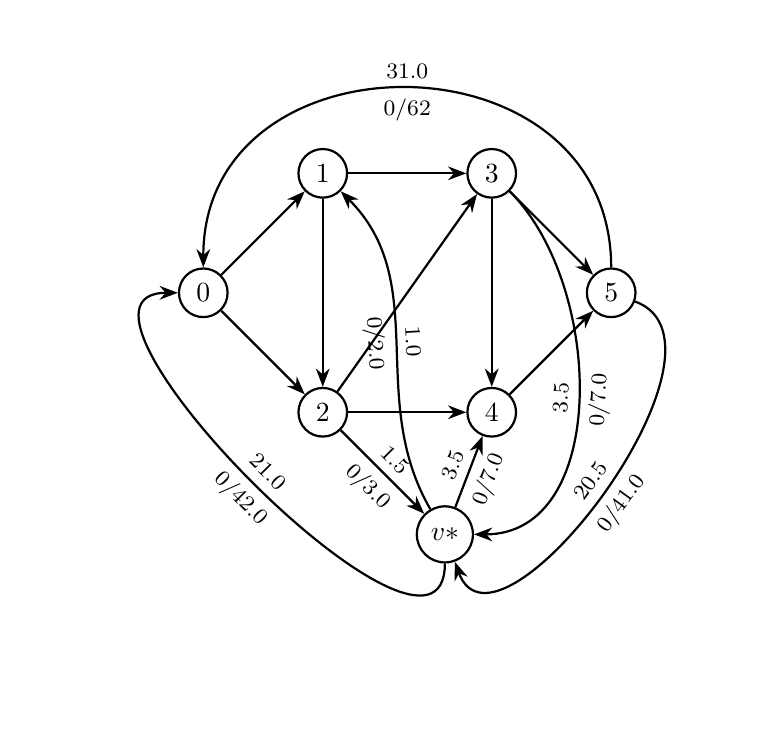
\begin{tikzpicture}[
    node distance={15mm},
    thick,
    main/.style = {
        draw,
        circle
    },
    myarrow/.style={
        -Stealth
    }
]
     
  \node[main] (0) {$0$};
  \node[main] (1) [above right=of 0] {$1$};
  \node[main] (2) [below right=of 0] {$2$};
  \node[main] (3) [right=of 1] {$3$};
  \node[main] (4) [right=of 2] {$4$};
  \node[main] (5) [below right=of 3] {$5$};
  \node[main] (6) [below right=of 2] {$v*$};
  \draw[myarrow] (0) to (1);
  \draw[myarrow] (0) to (2);
  \draw[myarrow] (1) to (3);
  \draw[myarrow] (1) to (2);
  \draw[myarrow] (2) to (3);
  \draw[myarrow] (2) to (4);
  \draw[myarrow] (3) to (4);
  \draw[myarrow] (3) to (5);
  \draw[myarrow] (4) to (5);
  \draw[myarrow] (5) to[out=90,in=90,looseness=1.5] node[font=\footnotesize,sloped,midway, below] {0/62} node[font=\footnotesize,sloped,midway, above] {31.0} (0);
  \draw[myarrow] (6) to[out=-90,in=180] node[font=\footnotesize,sloped,midway, below] {0/42.0} node[font=\footnotesize,sloped,midway, above] {21.0} (0);
  \draw[myarrow] (6) to[out=120,in=-45] node[font=\footnotesize,sloped,midway, below] {0/2.0} node[font=\footnotesize,sloped,midway, above] {1.0} (1);
  \draw[myarrow] (2) to node[font=\footnotesize,sloped,midway, below] {0/3.0} node[font=\footnotesize,sloped,midway, above] {1.5} (6);
  \draw[myarrow] (3) to[out=-45,in=0] node[font=\footnotesize,sloped,midway, below] {0/7.0} node[font=\footnotesize,sloped,midway, above] {3.5} (6);
  \draw[myarrow] (6) to node[font=\footnotesize,sloped,midway, below] {0/7.0} node[font=\footnotesize,sloped,midway, above] {3.5} (4);
  \draw[myarrow] (5) to[out=-20, in=-70] node[font=\footnotesize,sloped,midway, below] {0/41.0} node[font=\footnotesize,sloped,midway, above] {20.5} (6);
\end{tikzpicture}
\end{document}
